\section{Using your custom image}
\uninuvola offers the opportunity to load and use your custom image into the server. In this way you can import images from other services and test your own image while building it ( you can find a brief guide on how compile your own image in Section \ref{image_creation}). \\

In  the image selection page, Figure  \ref{image_selection}, you can select the option \textit{Other images} and select \textit{Other}. You will need to type the docker image name in the \textit{Custom image} section using the following formalism: \textit{image\_name:version}. 

\subsection{Example: Pangeo Notebook}
As an example of customised notebook we will import the Pangeo notebook. Pangeo is a community promoting open, reproducible, and scalable Big Data geoscience. Figure \ref{img:pangeo} shows a snippet of the \href{https://hub.docker.com/r/pangeo/pangeo-notebook/tags}{Dockerhub project page}:the page's  title corresponds to the \textit{image\_name}, with each available tag shown in boxes. These information can be found on the right side of each box. 

\begin{figure}[htbp]
    \centering
    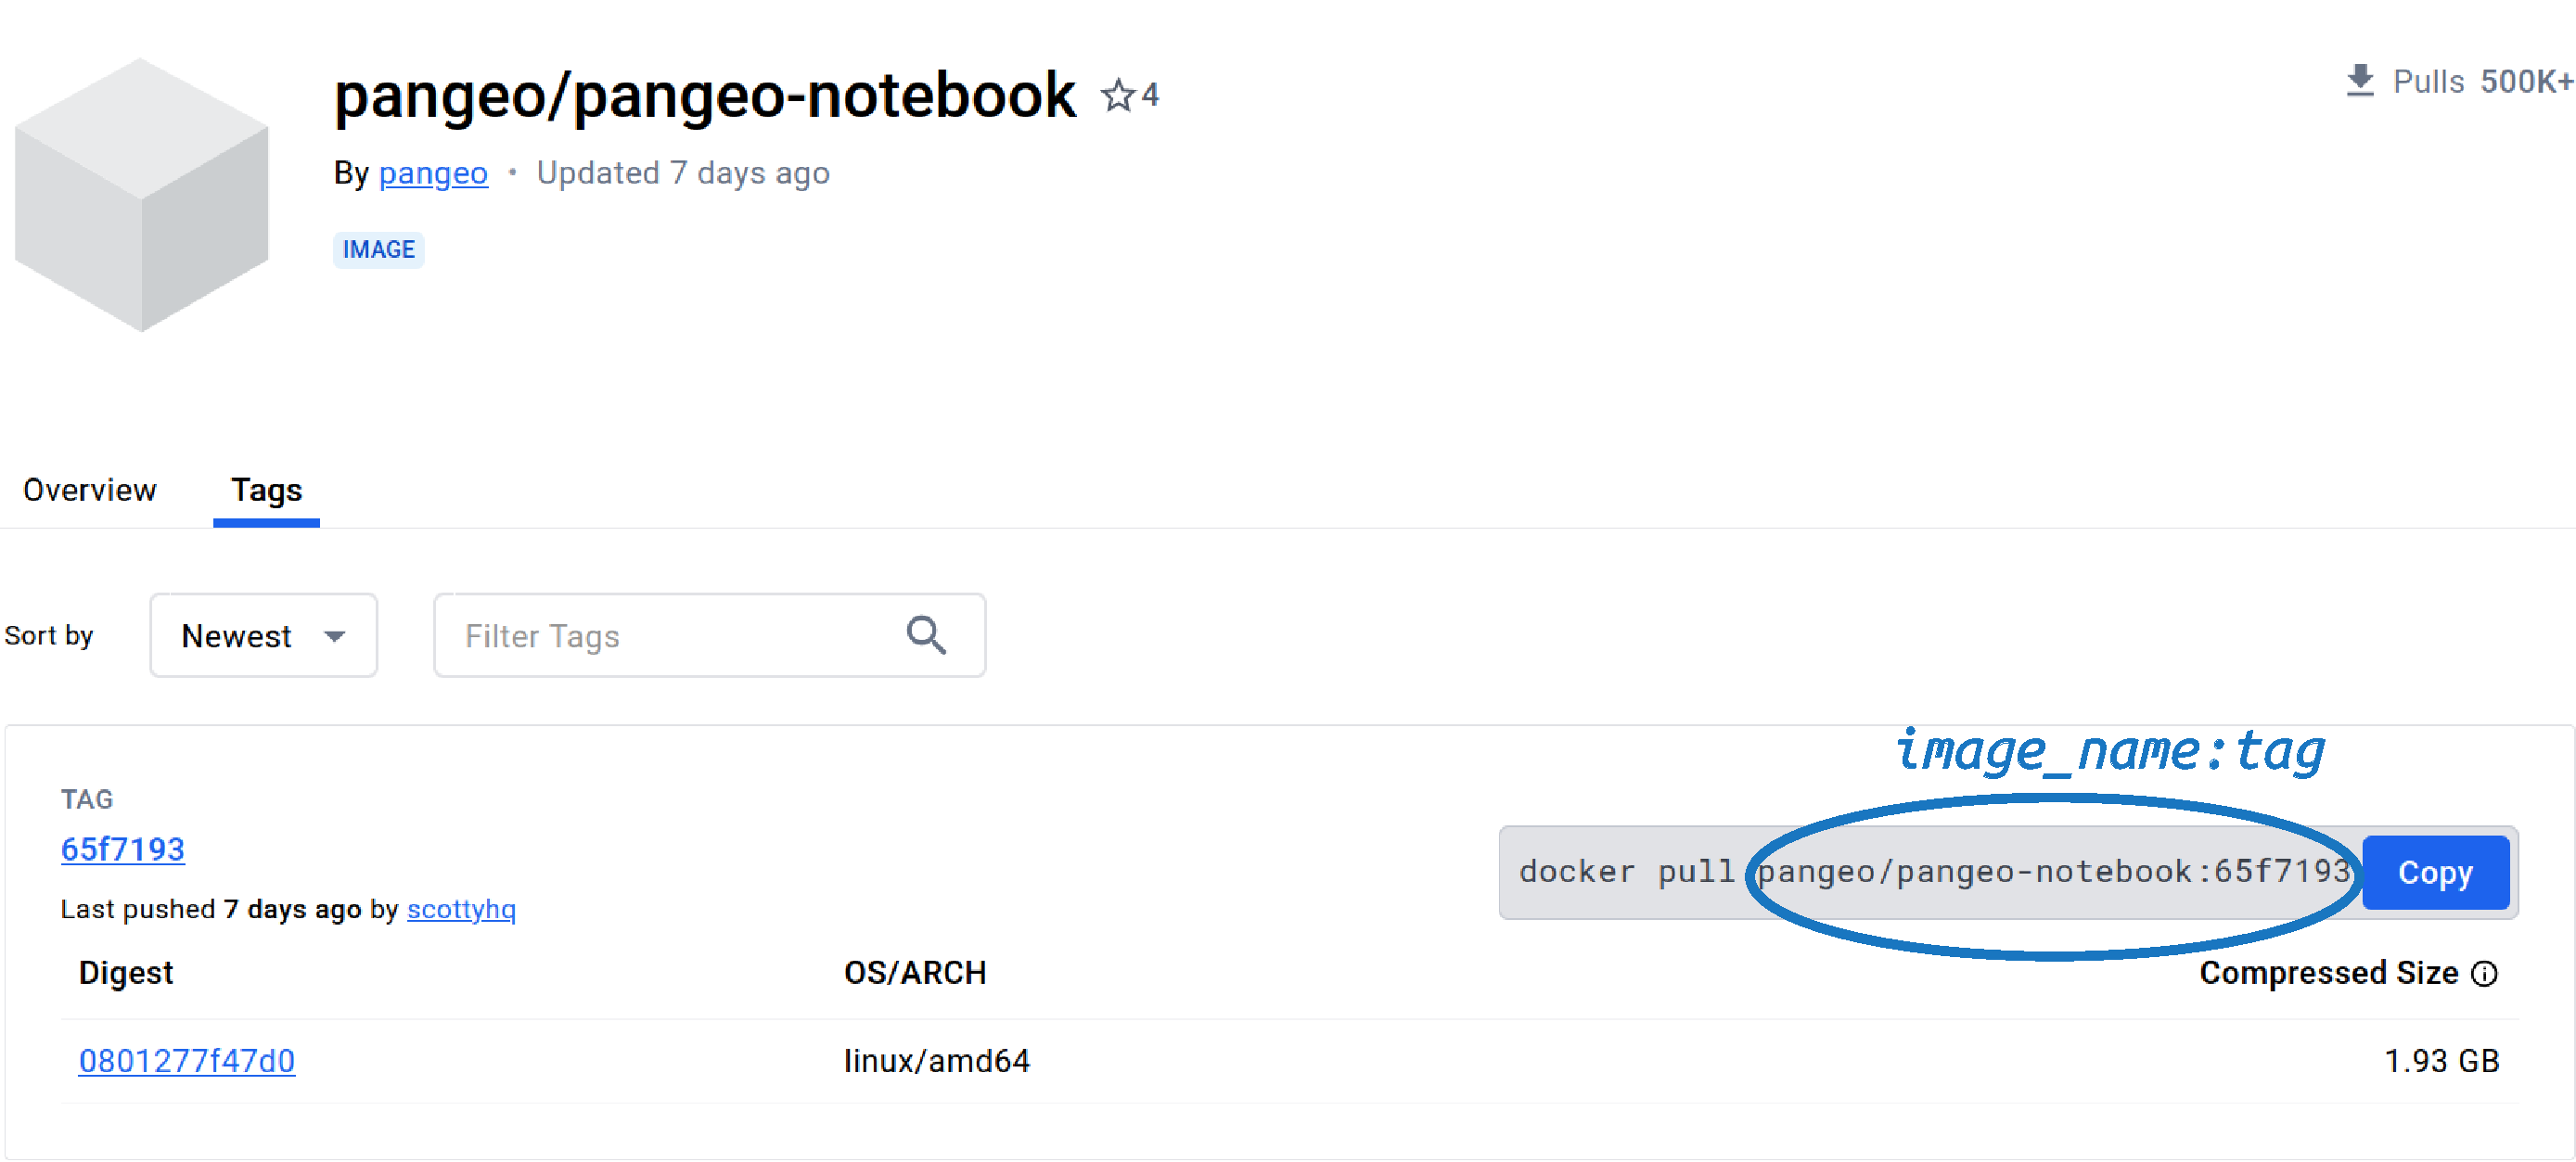
\includegraphics[width=0.9\textwidth]{figures/pangeo.pdf}
    \caption{Dockerhub page for the \href{https://hub.docker.com/r/pangeo/pangeo-notebook/tags}{Pangeo project}. }
    \label{img:pangeo}
\end{figure}

These information are inputted into the custom image cell, as it seen in Figure \ref{img:pangeo_opne}.

\begin{figure}[htbp]
    \centering
    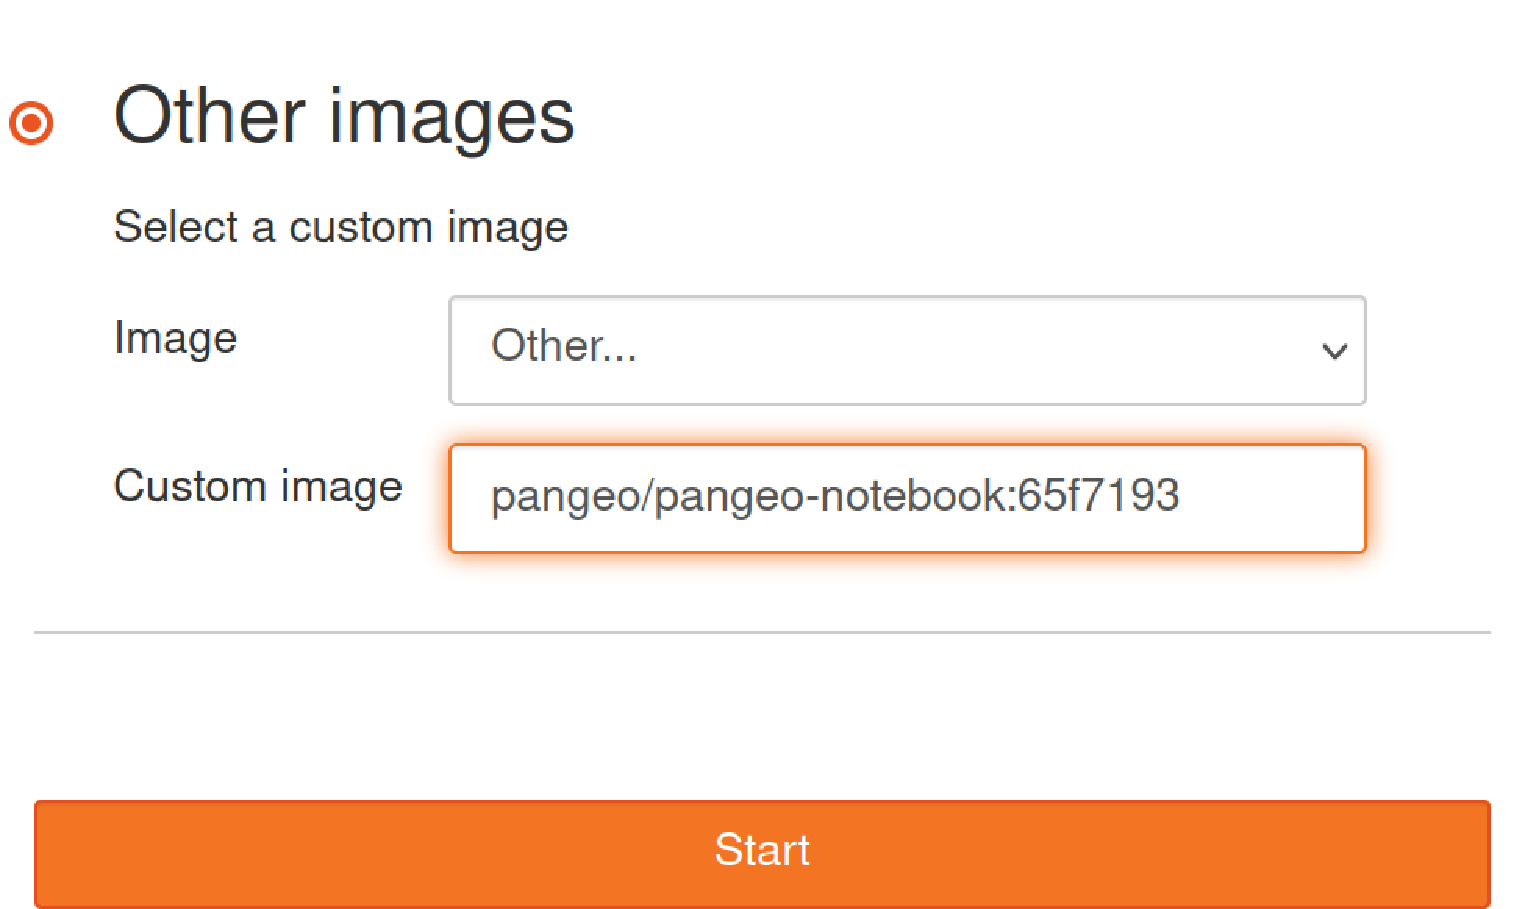
\includegraphics[width=0.75\textwidth]{figures/pangeo_open.pdf}
    \caption{Practical example of custom image selection. }
    \label{img:pangeo_opne}
\end{figure}


%[]


% DA QUELLO CHE VEDO POSSIAMO CARICARE IMMAGINI SOLO DA DOCKERHUB, CHE POTREBBE ESSERE UN PROBLEMA(?). iMMAGINI DA QUAY.IO NON SONO CARICATE. ALTRA COSA DA CONTROLLARE: L'IMMAGINE DEVE ESSERE BASATA SU JHUB GIUSTO? I DOCKER DI FEDORA E R NON PAIONO LAVORARE  